\Author{\daAuthorOne}

\todo{Bilder bearbeiten, weil gerade keine Daten angezeigt werden beim deployten Admin-Panel}

The Admin Panel is a Flutter-based administrative dashboard that allows the administrator to efficiently manage all addresses in the application, to plan  future "Sternsinger" events and assign designated zones to groups. This zoning ensures organized distribution of participants. It enables CRUD (Create, Read, Update, Delete) operations on addresses, streets and zones. These features make it easy for the administrator to quickly address issues and make changes to areas that participants need to visit.

\subsection{Navigation}

\noindent

\begin{figure}[H]

\begin{minipage}{0.58\textwidth}
    \setstretch{1.5} % Erhöht den Zeilenabstand
    The file \texttt{AdminNavigation} is used to manage the navigation between the different pages of the Admin Panel. The navigation can be done via a sidebar on the left which can be set visible via a button on the top left of the screen. The widget contains a list of pages and maintains an internal state (\texttt{indexState}) to keep track of the currently selected page. Whenever a page is selected in the sidebar, the \texttt{indexState} is updated and the corresponding page is displayed.
    \end{minipage}
    \hfill
    \begin{minipage}{0.38\textwidth}
    \centering
    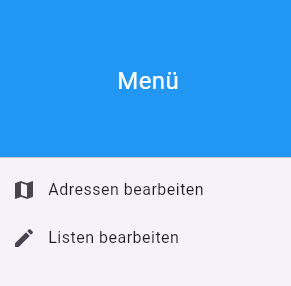
\includegraphics[width=0.7\linewidth]{images/AdminPanel/Menu.png}
    \caption{Navigation im Admin-Panel}
    \label{fig:adminpanel_navigation}
\end{minipage}

\end{figure}



\subsection{Pages}

\begin{subsubsection}{AddressPage}

The Page \texttt{AddressPage} displays all addresses in the database. With it, the administrator can add, edit and delete addresses into the database. All addresses are shown eather in the \texttt{MapComponent} or the \texttt{DatabaseViewComponent} on the right. On the left of the page are \texttt{InputFields}, which are used to enter new information about a new address, or edit an existing one. Overlapping the \texttt{MapComponent} there are:
\begin{itemize}
  \item a field to filter the addresses displayed
  \item a button with a dropdown menu to select an edit a street
  \item a switch to toggle between the \texttt{MapComponent} and the \texttt{DatabaseViewComponent}
  \item a information box on the bottom right corner to display the coordinates of the mouse pointer on the map
  \item another information box on the bottom left corner to display the selected coordinates, which is only visible when the admin presses the map
\end{itemize}

\begin{figure}[H]
    \centering
    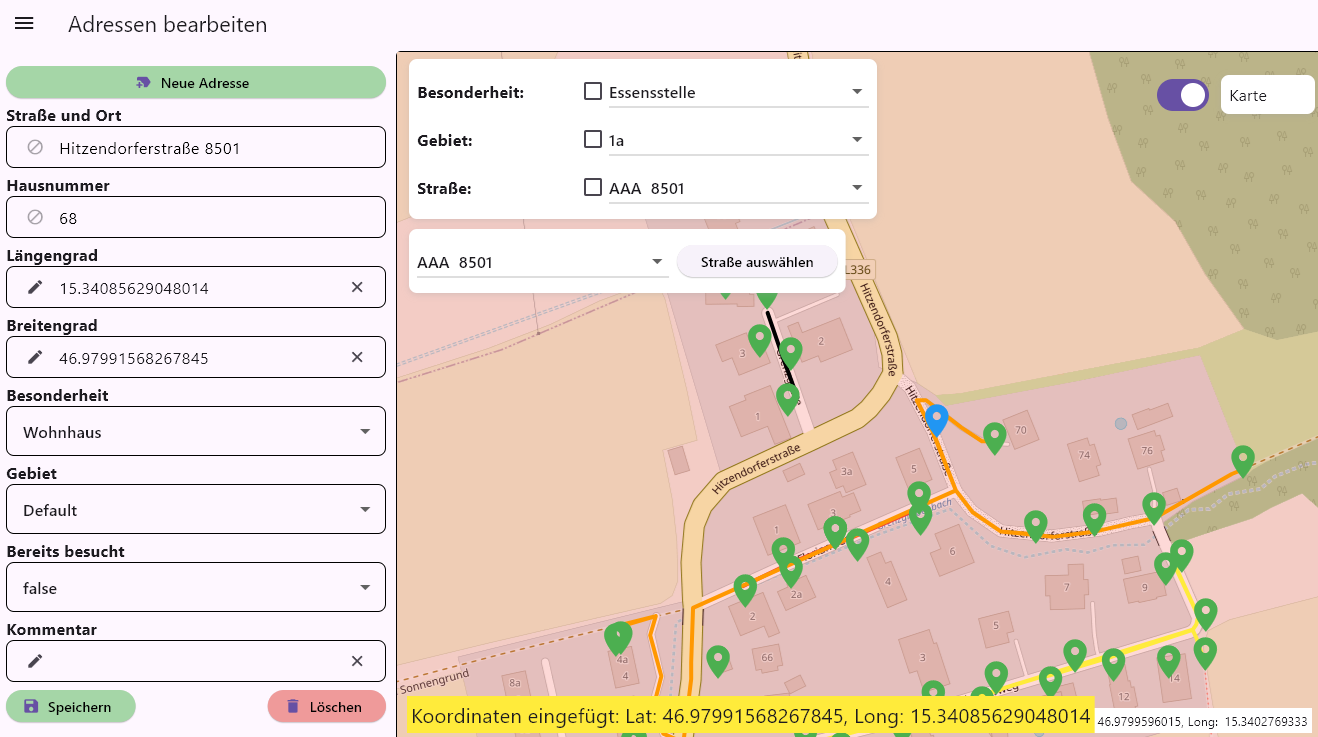
\includegraphics[width=0.9\linewidth]{images/AdminPanel/AddressPage.png}
\end{figure}
\end{subsubsection}


\paragraph{Add Address}


\paragraph{Edit Address}

\paragraph{Delete Address}


\begin{figure}[H]
    \setstretch{1.5} % Erhöht den Zeilenabstand
    \centering
    \begin{minipage}{0.55\textwidth} % Linke Seite für den Text
        \paragraph{Filter}
        With the Filter field, the administrator can filter the addresses displayed. It contains three dropdown menus to set the filter criteria, with one checkbox for each to toggle them. These filters can be combined as desired. 
    \end{minipage}
    \hfill 
    \begin{minipage}{0.4\textwidth} % Rechte Seite für das Bild
        \centering
        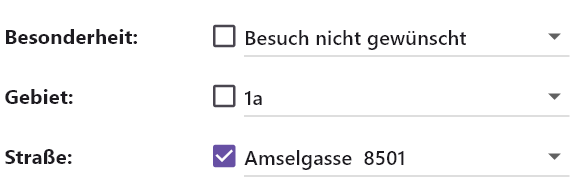
\includegraphics[width=\linewidth]{images/AdminPanel/FilterField.png}
        \caption{Filter field in AddressPage}
        \label{fig:adminpanel_filter}
    \end{minipage}
\end{figure}

The filter is passed and applied to the \texttt{MapComponent} and the \texttt{DatabaseViewComponent}. The criteria and their enabled/disabled state are managed by the following variables in the \texttt{AddressPage} class.
\lstset{style=mycsharp, caption=Filter variables in AddressPage}
\begin{lstlisting}
    bool specialFeatureFilter = false;
    bool areaFilter = false;
    bool streetFilter = false;
    
    String selectedStreetFilter = "";
    String selectedSpecialFeatureFilter = "";
    String selectedAreaFilter = "";
\end{lstlisting}

This is an example of how a \texttt{FilterRow} is defined in the \texttt{AddressPage} class (\ref{fig:FilterRow}):
\lstset{style=mycsharp, caption=FilterRow in AddressPage}
\begin{lstlisting}
    FilterRow(
        label: "Besonderheit:",
        tooltipMessage: "Besonderheitsfilter aktivieren/deaktivieren",
        filterValue: specialFeatureFilter,
        onFilterChanged: (bool? newValue) {
          setState(() => specialFeatureFilter = newValue ?? false);
        },
        selectedValue: selectedSpecialFeatureFilter,
        items: specialFeatureTextList,
        onDropdownChanged: (String? newValue) {
          setState(() => selectedSpecialFeatureFilter = newValue ?? "");
        },
      ),
\end{lstlisting}




 

\subsubsection{ListEditPage}


\subsection{Components}


\subsubsection{MapComponent}

\subsubsection{DatabaseViewComponent}

\subsubsection{PDFSaver}

\subsubsection{AdminAddressProvider}

\subsubsection{CustomHttpClient}

\subsection{Models}

\subsubsection{AreaWithBorder}

\subsubsection{ScreenItem}

\subsection{Widgets}

\subsubsection{InputField}

\subsubsection{FilterRow}
\label{fig:FilterRow}